\section{Design}
In this section, we describe the design of \tool{} by focusing on
how our design solves the three challenges discussed in the previous
section.

\subsection{Workflow}
%\subsection{Overview}
The shortcomings of the existing work inspire us to design a new tool to detect
and quantify information leakage vulnerabilities in binaries. The tool has three
steps. First, we run the target program with the concrete input 
(sensitive information) under the dynamic binary instrumentation (DBI) frameworks
to collect the execution traces. After that, we run the symbolic execution 
to capture the fined-grained semantic information of each secret-dependent 
control-flow transfers and data-accesses. 
Finally we run the Markov Chain Monte Carlo (MCMC) to estimate the 
information leakage. 

\begin{figure*}[ht]
    \centering
    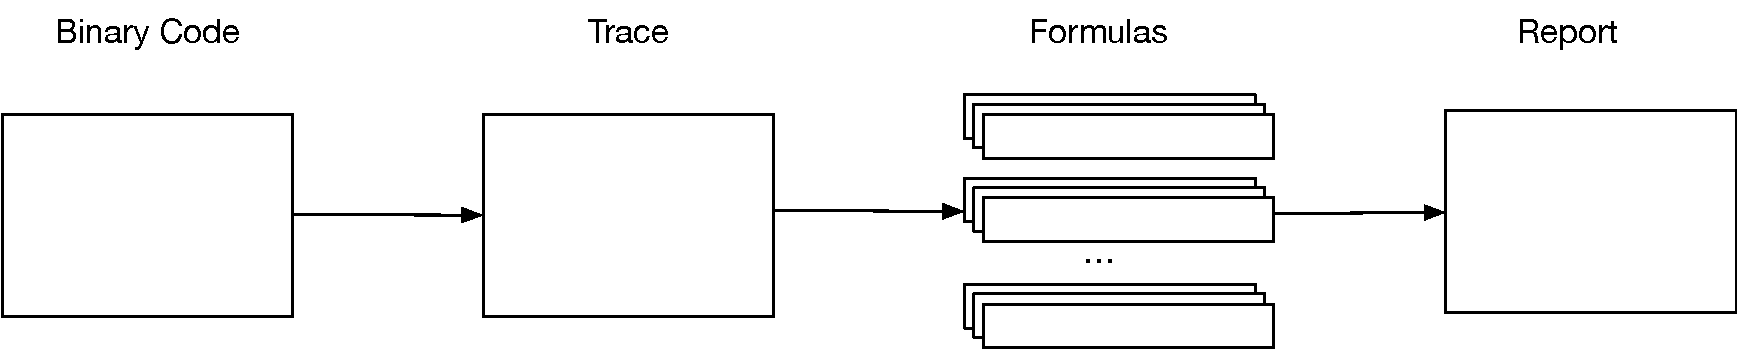
\includegraphics[width=\columnwidth]{./figures/workflow.pdf}
    \caption{The workflow of \tool{}. \fixme{redraw the figure. i will give you the instruction.}}
    \label{fig:Test}
\end{figure*}

\begin{enumerate}
    \item \textit{Execution trace generation.} The design goal of \tool\ is to
    estimate the information leakage as precisely as possible. Therefore,
    we sacrifice the soundness for the precision in terms of program analysis.
    Previous works~\cite{203878,217537} have demonstrated the effectiveness of the
    dynamic program analysis. We run the target binary under the dynamic binary
    instrumentation (DBI) to record the execution trace and the runtime information.
    \item \textit{Instruction level symbolic execution.} We model the 
    attacker's observation about the side-channel vulnerabilities with math
    formula. Each formula capture the fined-grained information between the input secrets
    and the leakage site. For the consideration of precision and performance, 
    we remove the intermediate language(IR) layer of the symbolic execution. 
    Also, the engine only symbolically execute the instruction that might be affected the
    input key. The above design significantly reduces the overhead of the symbolic
    execution, which make the tool scales to real-world programs.
    \item \textit{Leakage estimation.} We transfer the information leakage quantification
    problem into the problem of counting the number of assignments that satisfy the formulas
    which models the observations from attacker. We propose a markov monte carlo method to 
    estimate the number of satisfied solutions. With the help of Chebyshev's Inequality,
    we also give the an error estimate with the probability.
\end{enumerate}


\subsection{Trace Logging}
The trace information can be logged via some emulators (e.g., QEMU) or 
dynamic binary instrumentation tools (DBI). 
We run a program with the concrete input under the DBI to record the
execution trace.
The trace data has the following information:
\begin{itemize}
    \item Each instruction mnemonics and its memory address.
    \item The operands of each instruction and their concrete values during the 
          runtime.
    \item The value of eflags register. 
    \item The memory address and the length of the sensitive information.
     Most software developers stores sensitive information in an array,
     a variable or a buffer, which means that those data is stored in a contiguous 
     area in the memory. We use the symbol information in the binary to track the 
     address in the memory.
\end{itemize}

\subsection{Instruction Level Symbolic Execution}
\label{InstructionSE}
The main purpose of the step is to generate 
constraints of the input sensitive information from the execution trace. 
If we give the target program a new input which 
is different from the origin input that was used 
to generate the execution trace but still satisfies those constraints,
the new execution trace still have the same control flow and 
data access patterns. 

The tool runs the symbolic execution on the top of the execution traces.
At the beginning of the symbolic execution, the tool creates fresh 
symbols for each byte in the sensitive buffer. For other data in the 
register or memory at the beginning, we use concrete values from the 
runtime information collected during the runtime. 
During the symbolic execution for each instruction, 
the tool updates every variable in the memory and registers with a
math formula. The formula is made up with concrete values and 
the input key as the symbols accumulated through the symbolic execution.
For each formula, the tool will check weather it can be reduced
into a concrete values (e.g., $k_1+12-k_1 = 12$ ). 
If so, the tool will only use the concrete values in the 
following symbolic execution.

\subsubsection{Verification and Optimization}
We run the symbolic execution(SE) on the top of x86 instructions.
In other words, we don’t rely on any intermediate languages to 
simplify the implemetation of symbolic execution. 
While the implementation itself 
has a lot of benefits (Better performance, accurate memory model), 
we need to implement the symbolic execution 
rules for each X86 instruction. 
However, due to the complexity of X86, it is inevitable to make mistakes. 
Therefore, we verify the correctness of the SE engine during the execution. 
The tool will collect the runtime information (Register values, 
memory values) and compare them with the formula generated from the 
symbolic execution. Whenever the tool finishes the symbolic execution 
of each instruction, the tool will compare the formula for each symbol 
and its actual value. If the two values don't match, we check the code
and fix the error. Also, if the formula doesn't contain any symbols,
the tool will use the concrete value instead of symbolic execution.

\subsubsection{Secret-dependent control-flows}
An adversary can infer sensitive information from secret dependent control-flows. 
There are two kinds of control-transfer instructions: the unconditional 
control-transfer instructions and the conditional transfer instructions.
The unconditional instructions, like CALL, JUMP, RET transfer control
from one code segment location to another. Since the transfer is 
independent from the input sensitive information, an attacker was 
not able to infer any sensitive information from the control-flow. 
So the unconditional control-transfer doesn't leak any information 
based on our threat model. During the symbolic execution, 
we just update the register information and memory cells with 
new formulas accordingly.

The conditional control-flow transfer instructions, like conditional jumps,
depending on CPU states, may or may not transfer control flows.
For conditional jumps, the CPU will test if certain condition flag 
(e.g., CF = 0, ZF =1) is met and jump to the certain branches respectively.
The symbolic engine will compute the flag and represent the flag 
in a symbol formula. Because we are running on a symbolic execution 
on a execution trace, we know which branch is executed.
If a conditional jump uses the CPU status flag, we will generate 
the constraint accordingly.

\begin{figure}[ht]
      \centering
      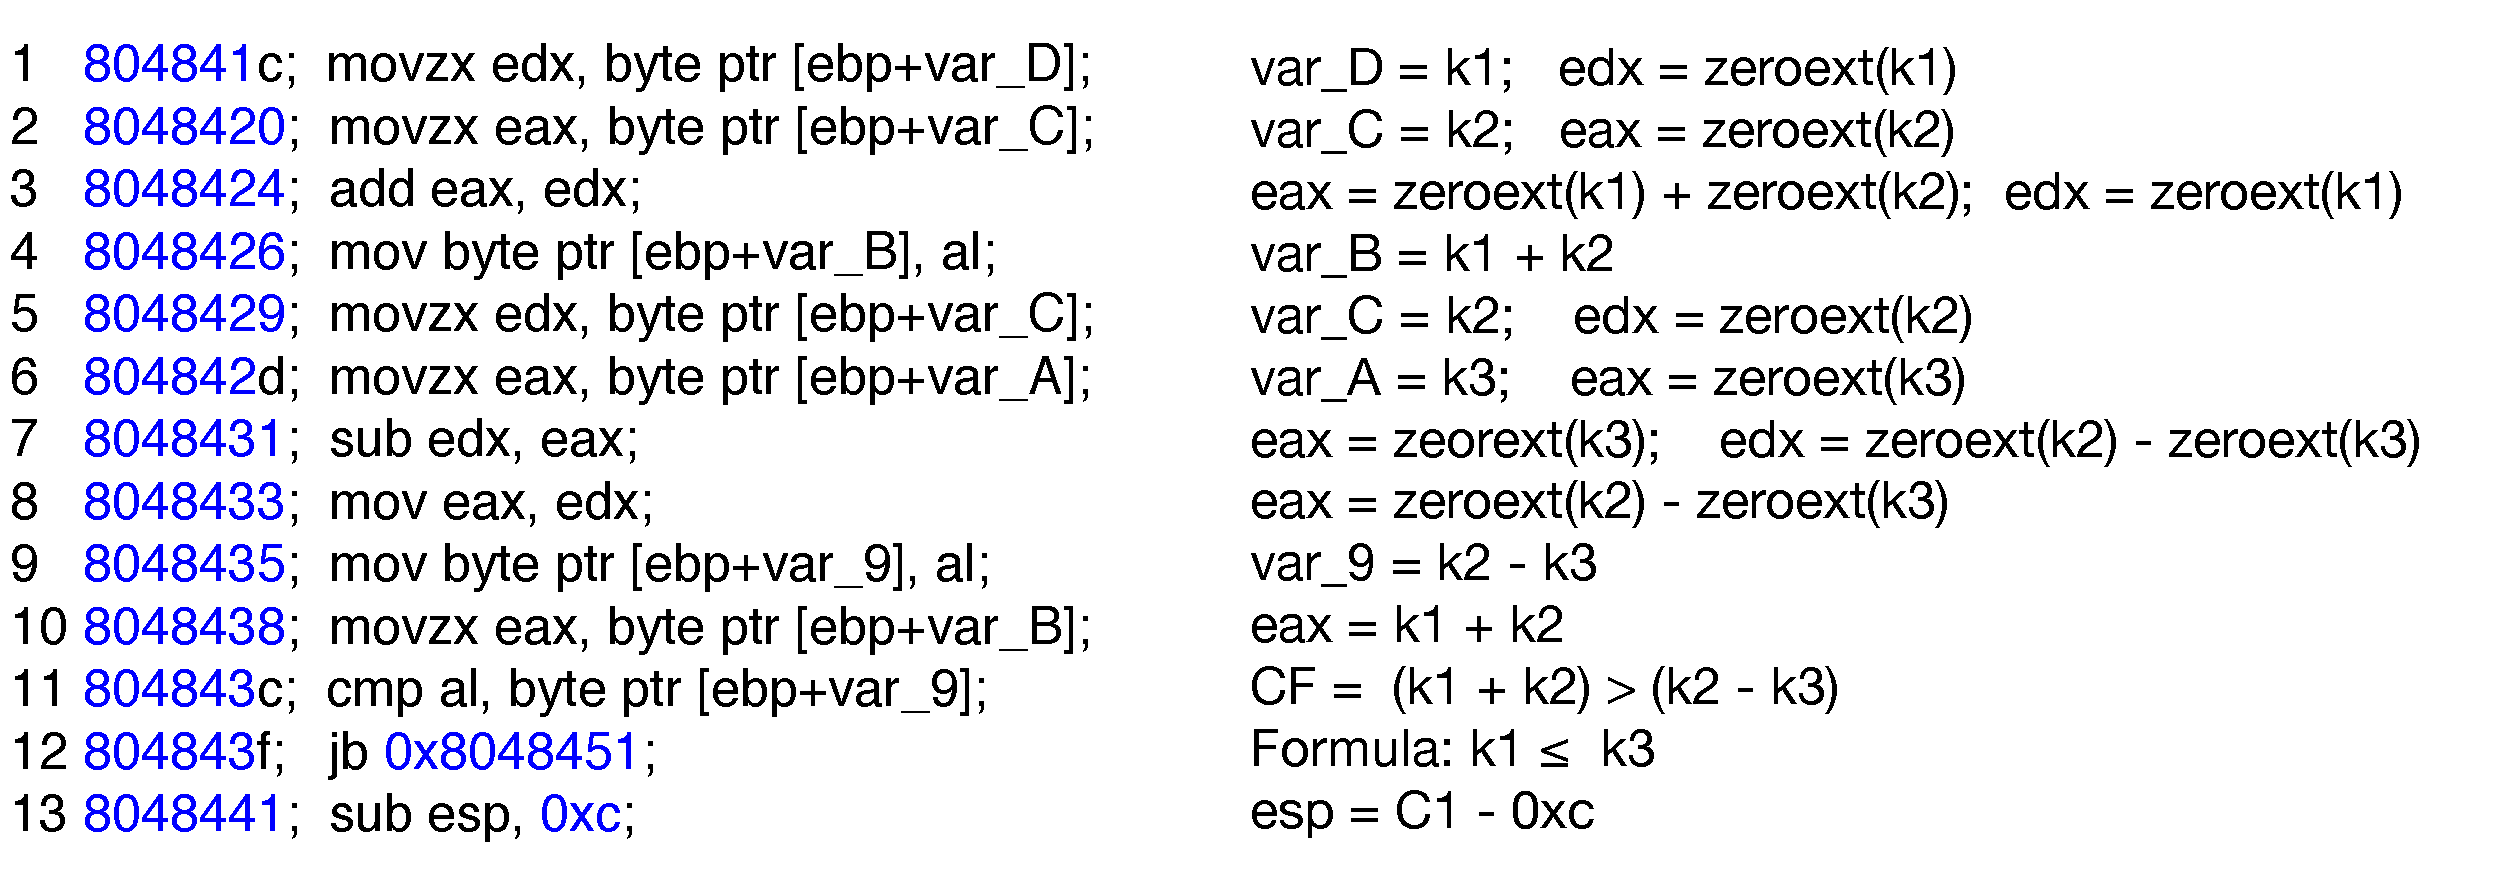
\includegraphics[width=\columnwidth]{./figures/secretCF.pdf}
      \caption{The workflow of \tool{}}
      \label{fig:Test}
  \end{figure}

For examples,

\begin{lstlisting}
...
0x0000e781      add dword [local_14h], 1
0x0000e785      cmp dword [local_14h], 4
0x0000e789      jne 0xe7df
0x0000e78b      mov dword [local_14h], 0
...
\end{lstlisting}

At the beginning of the instruction segment, the value at the 
address of local14h can be written as $F(\vec{K})$. At the address e785, 
the value will be updated with $F(\vec{K})+1$. Then the code compares 
the value with 4 and use the result as a conditional jump. 
Based on the result, we can have the following formula:

$$F(\vec{K}) + 1 = 4$$

The formula, together with the memory address (0xe789) is store
as a \textit{formula tuple (address, formula)}. 
Each formula tuple represents one leakage site.

\subsubsection{Secret-dependent data access}
Like input-dependent control-flow transfers, an adversary can also infer 
sensitive information from the data access pattern as well. 
We try to find this kind of leakages by checking 
every memory operand of the instruction. We generate the memory addressing 
formulas. As discussed before, every symbols in the formula is the input key. 
If the formula doesn’t contain any symbols, the memory access is independent 
from the input sensitive information and won’t leak any sensitive information 
according to our threat model. Otherwise, we will generate the constraint for
the memory addressing. We model the memory address with a symbolic formula 
$F(\vec{K})$. 
Because we also have the concrete value of the memory address $Addr1$. 
Inspired by the work from~\cite{203878}, the formula can be written as:

$$F(\vec{K}) >> L = Addr1 >> L$$

The $L$ represents the minimum memory address granularity that an attacker 
can observe. For example, Flush and Reload can distinguish between different
cache lines, which means the value of L is 6.

\subsubsection{Information Flow Check}
\tool{} is designed to help software developers find and understand the 
side-channel vulnerabilities. To ease the procedure of fixing the bug,
we also track the information flow for each byte of the input
buffer. 
The step can be seen as the mutiple-tag taint analysis.
With the help of the information from symbolic execution, we can implement
a relative simple but relatively precise information flow track.
At the begining of the analysis, \tool{} keep a track for each byte 
in the original buffer. When \tool{} symbolically executes each
instruction in the trace, it will check every value read from
registers or memory. If the value is concrete, it means the
instruction has nothing to do with the original buffer.
If the value is a formula, it means the orginal information
pass through the instruction. Since each byte in the sensitive
buffer is represented as a symbol with a unique ID, \tool{} can
know which byte in the origin buffer actually goes through the
instruction.

\subsection{Information Leakage Estimation}

In this section, we present the alogorithm to calculate the information
leakage based on the definition~\ref{def}. 

\subsubsection{Problem Statement}
From the above step~\ref{InstructionSE}, we can generate the constraint 
for each unique leakage site on the execution trace.
The only variables in those constraints are the sensitive data represented
with $k_1, k_2, ... , k_n$. Suppose the address of the leakage site is $addr_i$,
we use $C_{addr_i}$ to denote the constraint. For multiple leakage sites, 
as each leakage site has one constraint, we can 
use the conjunction of those constraints to represent those leakage sites. 

According to the definition~\ref{def}, to calculate the amount of leaked 
information, the key is to calculate $\frac{|K|}{|K^o|}$. $K^o$ represents
the set that contains every input keys that satisfy the constraint. As the 
cardinality of $K$ is known, the key problem is to know the cardinality of
$K^o$. Suppose an attacker can observe $n$ leakage sites, and each leakage site has
the following constraints: $C_{addr_1}, C_{addr_2}, ..., C_{addr_n}$ respectively. 
The total leakage has the constraint 
$F_{c_{addr_1},c_{addr_2},...,c_{addr_n}} = C_{addr_1} \land C_{addr_2} \land C_{addr_3}
\land ... \land C_{addr_n}$. The problem of estimating the total leaked information 
can be transfered into the problem of counting the number of different solutions 
that satisfies the constraint $F_{c_{addr_1},c_{addr_2},...,c_{addr_n}}$. 

A native method for approximating 
the result is to pick $k$ elements from $K$ and check how many of them are also
contained in $K^o$. If $q$ elements are also in $K^o$. In expectation, we can
use $\frac{k}{q}$ to approximate the value of $\frac{|K|}{|K^o|}$.

However, as the discussion in ~\ref{MCreasons},
the above sampling method will typically fail in practice due to the following two problems:

\begin{enumerate}
      \item The curse of dimensionality. $F_{c1...cn}$ is the conjunction of many
      constraints. Therefore, the input variables of each constraints will also be 
      the input variables of the $F_(c1...cn)$. The sampling method will fail as 
      $n$ increases. For example, when $n$ equals to 2, the whole serach space is 
      a $256^2$ cube. If we want the distance between each points equals to 1,
      we need $256^2$ points. When $n$ equals to 10, we need $256^{10}$ points if we 
      still we want the distance between each points equals to 1. As a result, the 
      error of the result based on sampling method will increase exponentially with
      adding dimensions. 

      \item The number of satisfying assignments could be exponentially small.
      According to Chernoff bound, we need exponentially many samples to get 
      a tight bound. On an extreme situation, if the constraint only has one unique
      satisfying solution, the simple Monte Carlo method can't find the satisfying
      assignment after sampling many points.
\end{enumerate}

In regard to the above problems, we present our methods. First, we split 
$F_(c_{addr_1},c_{addr_2},...,c_{addr_n})$ into several independent constraint groups. After
that, we run random-walk based sampling method on each constraint.

\subsubsection{Maximum Independent Partition}

For a constraint $C_i$, we define the function $S$, which maps
the constraint into the set consisting of input symbols. For example, 
$S(k1 + k2 > 128) = \{k1, k2\}$.

\theoremstyle{definition}
\newtheorem{definition}{Definition}[section]

\begin{definition}[]
      \label{independentC}
      Given two constraints $C_m$ and $C_n$, we call them independent iff 
      $$S(C_m) \cap S(C_n) = \emptyset$$
\end{definition}

Based on the definition~\label{independentC}, we can split
the constraint $F_{c_{addr_1},c_{addr_2},...,c_{addr_n}}$ into several 
independent constraints. There are many partitions. For our project, 
we are interested in the following one.

\begin{definition}
      \label{Goodpartition}
      For the constraint $F_{c_{addr_1},c_{addr_2},...,c_{addr_n}}$ and 
      the constraint group
      $C_{g1}, C_{g2}, ..., C_{gm}$, we call  $C_{g1}, C_{g2}, ..., C_{gm}$
      is the maximum independent partition of $F_{c_{addr_1},c_{addr_2},...,c_{addr_n}}$ iff
      \begin{enumerate}
            \item $C_{g1} \land C_{g2} \land ... \land C_{gm} = F_{c_{addr_1},c_{addr_2},...,c_{addr_n}}$
            \item $\forall \quad i, j \in \{1, 2, 3, ..., m\} \quad \textrm{and} \quad 
                  i \neq j, \quad S(C_{gi}) \cap S(C_{gj}) = \emptyset $
            \item For any other partitions  $C_{g1}, C_{g2}, ..., C_{gn}$ satisfy 1) and
                  2), $m \geq n$    
      \end{enumerate}
      
\end{definition}

The reason we want a good partition of the constraints is that we want to 
reduce the dimensions. Consider the example in the previous section,
$$F: {k_1} = 1\land{k_2} = 2\land{k_3} = 3\land{k_4} = 4$$
The good partition of $F$ would be
$$C_{g1}: {k_1} = 1\quad C_{g2}: {k_2} = 2\quad C_{g3}: {k_3} = 3\quad C_{g4}: {k_4} = 4$$     
So instead of sampling in the four dimension space, we can
sample each constraint in the one dimension space and combine them
together with~\ref{mip-theorem} .
\newtheorem{theorem}{Theorem}[section]
\label{mip-theorem}
\begin{theorem}
      \label{IndependentConstraint}
$C_{g1}, C_{g2}, ..., C_{gm}$ is a maximum independent partition of $F_{c_1c_2...c_n}$.
$K_c$ is the input set that satisfies constrain $c$. We can have the following
equation in regard to the size of $K_c$
$$|K_{F_{c_{addr_1},c_{addr_2},...,c_{addr_n}}}| = |K_{C_{g1}}|*|K_{C_{g2}}|*...*|K_{C_{gn}}|$$
\end{theorem}

With the~\ref{IndependentConstraint}, we can transfer the problem of counting the number of 
solutions in a large constraint with high
dimensions into counting solutions of 
several small constraints. We apply the following algorithm to get the Maximum Independent Partition
of the $F_{c_{addr_1},c_{addr_2},...,c_{addr_n}}$.

\IncMargin{1em}
\begin{algorithm}[h]
\DontPrintSemicolon
\SetKwInOut{Input}{input}\SetKwInOut{Output}{output}
\Input{$F_{c_{addr_1},c_{addr_2},...,c_{addr_n}} = C_{{addr}_1} \land C_{{addr}_2} \land ... \land C_{{addr}_m}$}
\Output{The Maximum Independent Partition of $G = \{C_{g1}, C_{g2}  , ...,  C_{gm} \}$ }
\For{$i\leftarrow 1$ \KwTo $n$}
{
   $S_i$ $\leftarrow$ $S(C_{addr_i})$ \;
   \For{$C_{gi} \in G$} 
   {
   $S_{gi}$ $\leftarrow$ $S(C_{gi})$ \;
   $s$ $\leftarrow$ $S_i \cap S_{gi}$  \;
   \If{$s \neq \emptyset$}
   {
      $C_{gi} = C_{gi} \land C_{addr_i}$ \;
      $break$ \;
   }
   Insert $C_{{addr}_i}$ to $G$
   }
}
\caption{The Maximum Independent Partition}
\end{algorithm}
\DecMargin{1em}

\subsubsection{Random Walk based Sampling}

After we split the constraints into several small constrainst, we count
the number of solutions on each constraints. Even though the total serach
space has been reduced greatly after the previous step, this is still a
\#P problem. For our project, we apply the approximate counting instead of
exact counting for two reasons. First, we don't need to have a very precise
result of the exact number of total solutions. The information is defined with
a logarithmic function. We don't need to distinguish between a formual having
$10^{10}$ and $10^{10} + 10$ solutions.
Second, as the constraint could be very complicated. The exact model counting
approaches, like DPLL search, have difficulty scaling up to large problem sizes.

We apply the "counting by sampling" method, which isn't a brand new idea~\cite{10.1007/11499107_24,Wei2004TowardsES}. 
We implement and extend the \textit{SampleSAT}~\cite{10.1007/11499107_24} to count the number 
of solutions for our constrains. The basic idea is as followed: if
one can sample nearly uniformly from the solutions of $F$, then one
get a good estimate of the number of solutions of $F$. 

\textit{SampleSAT} interleaves
the biased random walk and Monte Carlo Markov Chain Moves (MCMC). The hybrid
approach makes \textit{SampleSAT} samples more uniformly to
approximately count the number of solutions. Random walk (RW) is a 
local search heuristic methods. We start the search from
the one concrete sensitive input. If the constraint ($C_gi$) is the conjunction
of several small constraints, we feed the input into each small constraint. If 
the input value doesn't satisfy the small constrains, we just choose one input 
variable using the heuristic method and generate a new random value for the variable.

The random walk move can reach the solutions from every domains.
However, the sampling is biased with the biased random walk. Therefore,
we also introduce the Metropolis moves with the random walk move.

%% the algorithm
\IncMargin{1em}
\begin{algorithm}
\SetAlgoLined
\DontPrintSemicolon

\KwIn{{The constraint $C_{gi}$}}    
\KwOut{{The number of assignments that satisfy $C_{gi}$ $|K_{Ci}|$}}

\SetKwProg{RW}{RandomWalk}{}{}
\SetKwProg{MM}{MetropolisMove}{}{}
$n$: the number of sampling times \;
$P$: a probability generator \;
$v$: the input assignment \;
$n_{s}$: the number of satisfying assignments \;
\For{$i\leftarrow 1$ \KwTo $n$} {
      $p$ $\leftarrow$ $P$ \;
      \If{$p \geq 0.5$}
      {
        $v$ $\leftarrow$ \RW{$v$} {}
      }
      \Else{
            $v$ $\leftarrow$ \MM{$v$} {}
      }
      \If{$v$ satisfies $C_{gi}$}
      {$n_{s}$ $\leftarrow$ $n_{s} + 1$}
}

\caption{SampleSAT sampling}
\end{algorithm}
\DecMargin{1em}


%% the algorithm

